\documentclass[usenames,dvipsnames,aspectratio=169]{beamer}
\usepackage{../common/prgBasics}

\title[Lecture 9.]{Programming basics}
\subtitle{(GKNB\_INTA023)}

\begin{document}

%1
\begin{frame}[plain]
  \titlepage
\end{frame}

%2
\begin{frame}{Sorting numbers}
  Task:
  \begin{itemize}
    \item Improve the existing bubble sort program! Let the user enter the numbers to be sorted! Finish reading the input by entering a negative number.
    \item Entering more numbers than the size of the array must be prevented.
  \end{itemize}
  Problems:
  \begin{itemize}
    \item The count of numbers should be known at compile time
    \item Undersized array $\to$ there will be no space for the data
    \item Oversized array $\to$ wasting the memory
    \item The oversized array causes the smaller problem.
  \end{itemize}
\end{frame}

%3
\begin{frame}[fragile]{Sorting numbers}
  \begin{columns}[T]
    \column{.45\textwidth}
      \begin{block}{Output1}
        \small
        \begin{verbatim}
Enter non-negative numbers
Number #1: 2
Number #2: 4
Number #3: 1
Number #4: 3
Number #5: -1
After sorting:
1       2       3       4    
\end{verbatim}
      \end{block}
    \column{.45\textwidth}
      \begin{block}{Output2}
        \small
        \begin{verbatim}
Enter non-negative numbers
Number #1: 5
Number #2: 4
Number #3: 3
Number #4: 2
Number #5: 1
After sorting:
1       2       3       4       5    
\end{verbatim}
      \end{block}
  \end{columns}
\end{frame}

%4
\begin{frame}{Sorting numbers}
  \begin{exampleblock}{\textattachfile{bubble5.c}{bubble5.c}}
    \lstinputlisting[style=c,linerange={3-3},numbers=left,firstnumber=3]{bubble5.c}
    \lstinputlisting[style=c,linerange={37-46},numbers=left,firstnumber=37]{bubble5.c}
  \end{exampleblock}
\end{frame}

%5
\begin{frame}{Sorting numbers}
  \begin{exampleblock}{\textattachfile{bubble5.c}{bubble5.c}}
    \lstinputlisting[style=c,linerange={5-16},numbers=left,firstnumber=5]{bubble5.c}
  \end{exampleblock}
\end{frame}

%6
\begin{frame}{Dynamic memory allocation}
  \begin{itemize}
    \small
    \item The programmer decides the lifetime of dynamic variables
    \item \texttt{stdlib.h} must be included
    \item Memory allocation:\\
      \begin{itemize}
        \item \texttt{void *malloc(size\_t size);} \\
          Allocates \texttt{size} bytes of memory and returns its address. The allocated area is \emph{uninitialized}.
        \item \texttt{void *calloc(size\_t nmemb, size\_t size);} \\
          Allocates and returns the address of a continuous memory area for an array containing \texttt{nmemb} elements, each of which requires \texttt{size} bytes of memory. The area is \emph{initialized to zeros}.
        \item \texttt{void *realloc(void *ptr, size\_t size);} \\
          Resizing the already allocated memory area without modifying the stored content.
      \end{itemize}
    \item The return value is NULL in case of an error $\to$ should be checked
    \item Freeing memory: \texttt{void free(void *ptr);}
    \item The same meory area cannot be freed several times
    \item Freeing NULL does not cause problems
  \end{itemize}
\end{frame}

%7
\begin{frame}{Sorting numbers}
  Tasks:
  \begin{itemize}
    \item Allocate memory dynamically for the array containing the numbers to be sorted
    \item Enter the count of numbers first, then allocate the required amount of memory and read the numbers
    \item Do not forget to free the allocated area as soon as possible
  \end{itemize}
\end{frame}

%8
\begin{frame}{Sorting numbers}
  \begin{exampleblock}{\textattachfile{bubble6.c}{bubble6.c}}
    \lstinputlisting[style=c,linerange={34-42},firstnumber=34]{bubble6.c}
  \end{exampleblock}
\end{frame}

%9
\begin{frame}{Sorting numbers}
  \footnotesize
  \begin{exampleblock}{\textattachfile{bubble6.c}{bubble6.c}}
    \lstinputlisting[style=c,linerange={4-13},firstnumber=4]{bubble6.c}
  \end{exampleblock}
\end{frame}

%10
\begin{frame}{Student register}
  Tasks:
  \begin{itemize}
    \item Record the names and grades of students (one grade per student)
    \item Read the number of students first, then allocate the required amount of memory to store an array of name-grade structures
    \item Allocate memory dynamically even for the names!
    \item Sort the list according to the names and display it
  \end{itemize}
\end{frame}

%11
\begin{frame}{Student register}
  \footnotesize
  \begin{exampleblock}{\textattachfile{students1.c}{students1.c}}
    \lstinputlisting[style=c,linerange={6-9},firstnumber=6]{students1.c}
    \lstinputlisting[style=c,linerange={72-81},firstnumber=72]{students1.c}
  \end{exampleblock}
\end{frame}

%12
\begin{frame}{Student register}
  \scriptsize
  \begin{exampleblock}{\textattachfile{students1.c}{students1.c}}
    \vspace{-.3cm}
    \lstinputlisting[style=c,linerange={27-45},firstnumber=27]{students1.c}
    \vspace{-.3cm}
  \end{exampleblock}
\end{frame}

%13
\begin{frame}{Student register}
  \begin{exampleblock}{\textattachfile{students1.c}{students1.c}}
    \lstinputlisting[style=c,linerange={47-57},firstnumber=47]{students1.c}
  \end{exampleblock}
\end{frame}

%14
\begin{frame}{Student register}
  \footnotesize
  \begin{exampleblock}{\textattachfile{students1.c}{students1.c}}
    \lstinputlisting[style=c,linerange={59-70},firstnumber=59]{students1.c}
  \end{exampleblock}
\end{frame}

%15
\begin{frame}{Student register}
  \begin{exampleblock}{\textattachfile{students1.c}{students1.c}}
    \lstinputlisting[style=c,linerange={20-25},firstnumber=20]{students1.c}
  \end{exampleblock}
\end{frame}

%16
\begin{frame}{Sorting numbers}
  \small
  Task:
  \begin{itemize}
    \item Make the usage of our earlier program more comfortable! 
    \item Instead of entering the quantity of numbers in advance, let a special value signal the end of input $\to$ negative value
  \end{itemize}
  Problem:
  \begin{itemize}
    \item[] How much memory should we allocate if we do not know the number of numbers?
  \end{itemize}
  Solution \#1:
  \begin{itemize}
    \item[] Allocate a small memory block initially and as soon as it is full double its size $\to$ minimizes the number of memory re-allocations (=fast) at the cost of at most half of the allocated area remains unused
  \end{itemize}
  Remark:
  \begin{itemize}
    \item[] Due to simplicity and brevity we assume that memory allocations are always successful
  \end{itemize}
\end{frame}

%17
\begin{frame}{Sorting numbers}
  \begin{exampleblock}{\textattachfile{bubble7.c}{bubble7.c}}
    \lstinputlisting[style=c,linerange={45-55},firstnumber=45]{bubble7.c}
  \end{exampleblock}
\end{frame}

%18
\begin{frame}{Sorting numbers}
  \fontsize{8}{9} \selectfont
  \begin{exampleblock}{\textattachfile{bubble7.c}{bubble7.c}}
    \vspace{-.3cm}
    \lstinputlisting[style=c,linerange={4-24},firstnumber=4]{bubble7.c}
    \vspace{-.3cm}
  \end{exampleblock}
\end{frame}

%19
\begin{frame}[fragile]{Sorting numbers}
  \fontsize{7}{8} \selectfont
  \begin{block}{Output}
    \begin{verbatim}
Enter non-negative numbers
      [Initial memory allocation]
      [Used: 0, Array size: 1]
Number #1: 6
      [Used: 1, Array size: 1]
Number #2: 5
      [Memory re-allocation]
      [Used: 2, Array size: 2]
Number #3: 4
      [Memory re-allocation]
      [Used: 3, Array size: 4]
Number #4: 3
      [Used: 4, Array size: 4]
Number #5: 2
      [Memory re-allocation]
      [Used: 5, Array size: 8]
Number #6: 1
      [Used: 6, Array size: 8]
Number #7: 0
      [Used: 7, Array size: 8]
Number #8: -1
After sorting:
0       1       2       3       4       5       6
\end{verbatim}
  \end{block}
\end{frame}

%20
\begin{frame}{Drawing rectangles}
  Task:
  \begin{itemize}
    \item Modify the rectangle drawing program similarly, too
    \item Memory allocation strategy \#2: if the allocated area is full, increase its size always with the same amount $\to$ minimizes the unused memory area at the cost of much re-allocations (=slow)
    \item The function allocating memory for the array returns the number of elements and writes the address of the array where its parameter points to
  \end{itemize}
  \begin{exampleblock}{\textattachfile{rectangle3.c}{rectangle3.c}}
    \scriptsize
    \vspace{-.3cm}
    \lstinputlisting[style=c,linerange={91-98},firstnumber=91]{rectangle3.c}
    \vspace{-.3cm}
  \end{exampleblock}
\end{frame}

%21
\begin{frame}{Drawing rectangles}
  \begin{exampleblock}{\textattachfile{rectangle3.c}{rectangle3.c}}
    \footnotesize
    \vspace{-.3cm}
    \lstinputlisting[style=c,linerange={60-75},firstnumber=60]{rectangle3.c}
    \vspace{-.3cm}
  \end{exampleblock}
\end{frame}

%22
\begin{frame}{Drawing rectangles}
  \begin{exampleblock}{\textattachfile{rectangle3.c}{rectangle3.c}}
    \scriptsize
    \lstinputlisting[style=c,linerange={76-91},firstnumber=76]{rectangle3.c}
  \end{exampleblock}
\end{frame}

%23
\begin{frame}[fragile]{Drawing rectangles}
  \begin{columns}[T]
    \column{0.75\textwidth}
      \begin{block}{Output 1/2}
        \tiny
        \begin{verbatim}
  Please enter the data of rectangles!
          [Initial memory allocation]
          [Used: 0, Array size: 2]
  X coordinate of the top left corner of rectangle #1 [0, 78] (exits to a negative value) 3
  Y coordinate of the top left corner rectangle #1 [0, 23] 3
  X coordinate of the bottom right corner rectangle #1 [4, 79] 6
  Y coordinate of the bottom right corner rectangle #1 [4, 24] 6
  Drawing character of rectangle #1: +
          [Used: 1, Array size: 2]
  X coordinate of the top left corner of rectangle #2 [0, 78] (exits to a negative value) 5
  Y coordinate of the top left corner rectangle #2 [0, 23] 5
  X coordinate of the bottom right corner rectangle #2 [6, 79] 8
  Y coordinate of the bottom right corner rectangle #2 [6, 24] 8
  Drawing character of rectangle #2: -
          [Used: 2, Array size: 2]
  X coordinate of the top left corner of rectangle #3 [0, 78] (exits to a negative value) 7
          [Memory re-allocation]
  Y coordinate of the top left corner rectangle #3 [0, 23] 7
  X coordinate of the bottom right corner rectangle #3 [8, 79] 10
  Y coordinate of the bottom right corner rectangle #3 [8, 24] 10
  Drawing character of rectangle #3: *
          [Used: 3, Array size: 4]
  X coordinate of the top left corner of rectangle #4 [0, 78] (exits to a negative value) -1
\end{verbatim}
      \end{block}
    \column{0.25\textwidth}
      \begin{block}{Output 2/2}
        \begin{verbatim}
   ++++                                                                         
   ++++                                                                         
   ++----                                                                       
   ++----                                                                       
     --****                                                                     
     --****                                                                     
       ****                                                                     
       ****
\end{verbatim}
      \end{block}
  \end{columns}
\end{frame}

%24
\begin{frame}{Matrices}
  \small
  Matrix: two dimensional array of data of the same type\\
  Only one dimensional arrays exist in C, but these can be embedded into each other $\to$ \\
  \qquad matrix = vector of vectors\\
  \begin{columns}[T]
    \column{0.5\textwidth}
      \hspace{.25cm} $A = \left[ \begin{array}{cccc}
                     11 & 12 & 13 & 14 \\
                     21 & 22 & 23 & 24 \\
                     31 & 32 & 33 & 34 \\
                   \end{array}
                \right]$
    \column{0.5\textwidth}
      \texttt{int A[3][4] = \{ \\
      \qquad \{11, 12, 13, 14\},\\
      \qquad \{21, 22, 23, 24\},\\
      \qquad \{31, 32, 33, 34\} \};}
  \end{columns}
  \begin{center}
    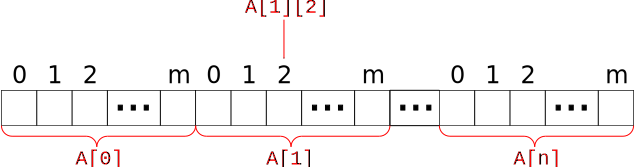
\includegraphics[width=0.8\textwidth]{matrix.pdf}
  \end{center}
  Adding up two matrices: $(A+B)[i,j] = A[i,j] + B[i,j]$, where $A$ and $B$ are $n\times m$ sized matrices.\\
\end{frame}

%25
\begin{frame}{Matrices}
  \begin{exampleblock}{\textattachfile{mtxAdd1.c}{mtxAdd1.c}}
    \scriptsize
    \lstinputlisting[style=c,linerange={4-20},firstnumber=4]{mtxAdd1.c}
  \end{exampleblock}
\end{frame}

%26
\begin{frame}{Matrices}
  \scriptsize
  \begin{exampleblock}{\textattachfile{mtxAdd1.c}{mtxAdd1.c}}
    \scriptsize
    \vspace{-.3cm}
    \lstinputlisting[style=c,linerange={21-40},firstnumber=21]{mtxAdd1.c}
    \vspace{-.3cm}
  \end{exampleblock}
\end{frame}

%27
\begin{frame}[fragile]{Matrices}
  \begin{block}{(A possible) output}
    \begin{verbatim}
11 12 13 14   33 49 36 12   44 61 49 26 
21 22 23 24 + 20 45 24 18 = 41 67 47 42 
31 32 33 34   19 10 11 42   50 42 44 76
\end{verbatim}
  \end{block}
  \vfill
  How can a matrix be passed to a function?\\
  \begin{exampleblock}{OK \checkmark}
    \texttt{void fn(int m[ROWS][COLS]) \{ //...\\
    void fn(int m[][COLS]) \{ //...\\
    void fn(int (*m)[COLS]) \{ //...}
  \end{exampleblock}
  \begin{alertblock}{Error X -- It is an array of pointers, not a matrix!}
    \texttt{void fn(int *m[COLS]) \{ //...}
  \end{alertblock}
\end{frame}

%28
\begin{frame}{Matrices}
  \begin{exampleblock}{\textattachfile{mtxAdd2.c}{mtxAdd2.c}}
    \vspace{-.3cm}
    \lstinputlisting[style=c,linerange={44-56},firstnumber=44]{mtxAdd2.c}
    \vspace{-.3cm}
  \end{exampleblock}
\end{frame}

%29
\begin{frame}{Matrices}
  \scriptsize
  \begin{exampleblock}{\textattachfile{mtxAdd2.c}{mtxAdd2.c}}
    \scriptsize
    \vspace{-.3cm}
    \lstinputlisting[style=c,linerange={4-23},firstnumber=4]{mtxAdd2.c}
    \vspace{-.3cm}
  \end{exampleblock}
\end{frame}

%30
\begin{frame}{Matrices}
  \scriptsize
  \begin{exampleblock}{\textattachfile{mtxAdd2.c}{mtxAdd2.c}}
    \scriptsize
    \lstinputlisting[style=c,linerange={25-42},firstnumber=25]{mtxAdd2.c}
  \end{exampleblock}
\end{frame}

%31
\begin{frame}{Matrices}
  \begin{columns}[T]
    \column{.5\textwidth}
      Problem:
      \begin{itemize}
        \item[] inflexible functions, the number of columns is fixed
      \end{itemize}
      \vfill
      Solution:
      \begin{itemize}
        \item create vectors dynamically (can be addressed by eg. \texttt{int*}), then 
        \item store their addresses in another dynamic vector (\texttt{int**}, array of pointers)!
      \end{itemize}
    \column{.5\textwidth}
      \includegraphics[width=\textwidth]{matrix2.pdf}
  \end{columns}
\end{frame}

%32
\begin{frame}{Matrices}
  \footnotesize
  \begin{exampleblock}{\textattachfile{mtxAdd3.c}{mtxAdd3.c}}
    \vspace{-.3cm}
    \lstinputlisting[style=c,linerange={55-70},firstnumber=55]{mtxAdd3.c}
    \vspace{-.3cm}
  \end{exampleblock}
\end{frame}

%33
\begin{frame}{Matrices}
  \begin{exampleblock}{\textattachfile{mtxAdd3.c}{mtxAdd3.c}}
    \footnotesize
    \lstinputlisting[style=c,linerange={5-19},firstnumber=5]{mtxAdd3.c}
  \end{exampleblock}
\end{frame}

%34
\begin{frame}{Matrices}
  \begin{exampleblock}{\textattachfile{mtxAdd3.c}{mtxAdd3.c}}
    \footnotesize
    \lstinputlisting[style=c,linerange={21-28},firstnumber=21]{mtxAdd3.c}
    \lstinputlisting[style=c,linerange={48-53},firstnumber=49]{mtxAdd3.c}
  \end{exampleblock}
\end{frame}

%35
\begin{frame}{Matrices}
  Alternative solution:
  \begin{itemize}
    \item we can mimic the stucture of ,,static'' arrays in memory, thus
    \item we allocate memory for a vector and map the elements of the matrix to this area
  \end{itemize}
  \begin{center}
    \includegraphics[scale=0.6]{matrix3.pdf}
  \end{center}
\end{frame}

%36
\begin{frame}{Matrices}
  \footnotesize
  \begin{exampleblock}{\textattachfile{mtxAdd4.c}{mtxAdd4.c}}
    \vspace{-.3cm}
    \lstinputlisting[style=c,linerange={44-59},firstnumber=44]{mtxAdd4.c}
    \vspace{-.3cm}
  \end{exampleblock}
\end{frame}

%37
\begin{frame}{Matrices}
  \scriptsize
  \begin{exampleblock}{\textattachfile{mtxAdd4.c}{mtxAdd4.c}}
    \vspace{-.3cm}
    \lstinputlisting[style=c,linerange={5-24},firstnumber=5]{mtxAdd4.c}
    \vspace{-.3cm}
  \end{exampleblock}
\end{frame}

\end{document}
